\documentclass[conference,11pt]{IEEEtran}
\usepackage{blindtext, graphicx}
\usepackage{flafter} %-kastan for tables mid-page

% *** GRAPHICS RELATED PACKAGES ***
%\usepackage[pdftex]{graphicx}
% *** MATH PACKAGES ***
\usepackage[cmex10]{amsmath}
\usepackage{amssymb}
\usepackage{float}
\DeclareMathOperator{\EX}{\mathbb{E}}
\DeclareMathOperator*{\minGAN}{min}
\DeclareMathOperator*{\maxGAN}{max}

% *** SPECIALIZED LIST PACKAGES ***
\usepackage{algorithmic}

% correct bad hyphenation here
\hyphenation{op-tical net-works semi-conduc-tor}

% fix some indentation issues
\setlength{\parskip}{1em}

\begin{document}
% paper title
\title{Facial Recognition with Information Maximizing Generative Adversarial Networks}

% author names and affiliations
% use a multiple column layout for up to three different
% affiliations
\author{\IEEEauthorblockN{Timothy Nguyen}
\IEEEauthorblockA{Department of Computer Science \\
Swarthmore College \\
Email: tnguyen5@swarthmore.edu} 
\and
\IEEEauthorblockN{Kastan Day}
\IEEEauthorblockA{Department of Computer Science \\
Swarthmore College \\
Email: kday1@swarthmore.edu}}

% make the title area
\maketitle

\begin{abstract}
%\boldmath
We present an extension on the earlier works of Information Maximizing Generative Adversarial Networks (InfoGAN) to perform facial recognition in an unsupervised manner.  Current state of the art techniques involve deep convolutional neural networks which manipulate and learn from individual pixel values.  InfoGAN seeks to continually generate realistic looking images provided a dataset and statistical variables to train on.  When given Categorical and Continuous variables of appropriate dimension, InfoGAN successfully distinguished among the different subjects in our training data.  
Additionally, the other higher dimension variables gave insight into how the network was able to discern between specific individuals by learning aspects such as facial structure, skin tone, or expression.

\end{abstract}

\section{Introduction}
Facial recognition is a common practice among countless technologies today.  Smart phones, web applications, robots, and even humans perform feature detection and recognition on a day to day basis.  However, these devices generally perform the task with many layers of convolutional neural networks, which extract raw pixel values and run complex algorithms on these pixels to distinguish among faces.

\begin{figure}[t]
%\centering
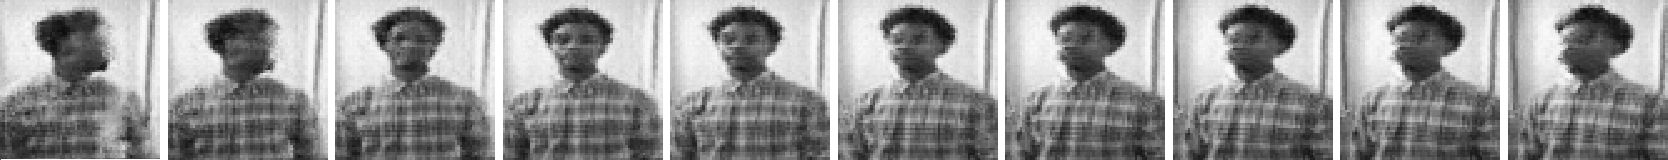
\includegraphics[width=\linewidth]{pictures/personal/rasheed-rotate-final.jpg}\vspace{2mm}
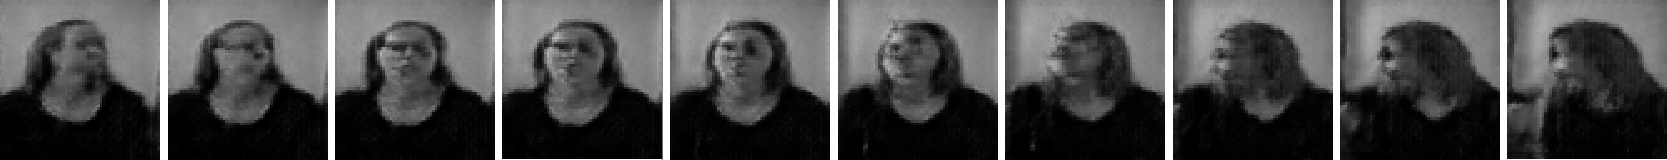
\includegraphics[width=\linewidth]{pictures/personal/lilly-rotate-final.jpg}\vspace{2mm}
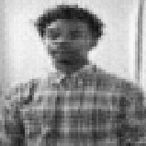
\includegraphics[width=.24\linewidth]{pictures/personal/bestRasheed.png}
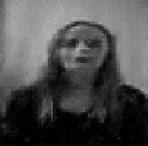
\includegraphics[width=.24\linewidth]{pictures/personal/bestLilly.png}
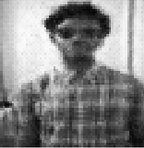
\includegraphics[width=.24\linewidth,trim={0 0 0 .22em},clip]{pictures/personal/bestRasheedGlasses.png}
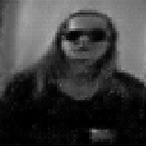
\includegraphics[width=.24\linewidth]{pictures/personal/bestLillyGlasses.png}
\caption{\textbf{Example of InfoGAN:}  A continuous code captured Rasheed's and Lilly's rotation (top) on a continuum from -1 to 1.  Below are 4 categorical representations of Rasheed and Lilly, one for each image. They are shown naturally, straight ahead, and straight ahead wearing sunglasses.}
\end{figure}

Instead of these traditional methods, we extend on a certain type of network, Generative Adversarial Networks (GAN) \cite{GAN}, to achieve our task.  Traditional GANs consist of two networks, a discriminator and a generator.  The discriminator aims to discern between real images, which our dataset provides, and generated images, which the generator network produces.  These two networks compete in this co-evolutionary arms race, where each network continually tries to best its competitor.  The objective is to learn a generative distribution of data through a two player minimax game, i.e. finding the Nash Equilibrium.  The generator produces increasingly realistic images that match the dataset, while the discriminator becomes increasingly skilled at discerning between these images.  The GAN co-evolutionary process can be thought of as a person attempting to print counterfeited currency (generator) and a bank attempting to accept genuine currency (discriminator) where they label currency (generated images) as real or fake. The knowledge of which currency the bank accepts is fed back to the counterfeiter who attempts to produce more realistic currency.

Naturally, we would want to expand on GAN by learning a conditional generative distribution, however, this variant, called CGAN \cite{CGAN}, must be given those conditionals manually to bootstrap learning.  These conditionals are either image labels or other auxilliary input.  CGAN defeats the purpose of unsupervision since we are providing explicit information about the training data.  Therefore, we extend on a variant known as InfoGAN \cite{infoGAN}, or Information Maximization Generative Adversarial Networks, to perform facial recognition in an unsupervised way.  InfoGAN attempts to learn those conditionals automatically by incorporating a third neural network, which aims to maximize mutual information between the provided variables and datasets.

We provide our network with facial datasets that contain many images of the same person.  InfoGAN works by trying to generate images that fit the provided input variables.  For example, we may specify a Categorical variable of dimension two, in which the network could learn the difference between between two subjects, or, of dimension 5, where it may learn different features like wearing glasses, or striking a different pose (Figure 1).  We may also specify a Continuous variable, in which it could learn to fit a continuous range of a subject's rotation.

The fundamentals of the network remain consistent with how InfoGAN was originally presented.  Their experiment, however, did not provide datasets which contained similar traits.  The facial dataset they trained on was the CelebA dataset, consisting of over 200,000 images of different faces.  Although this gives infoGAN a broad spectrum of examples to learn from, it won't empirically demonstrate that it learned traits essential for facial recognition.

We hypothesize that InfoGAN will succeed in learning to differentiate between people if given a proper dataset.  InfoGAN should be able to learn differences in face structure, hair styles, skin tones, etc. and apply that knowledge to generate unique images of each particular person.  These are the same traits that humans use to recognize and classify similar objects.  Ultimately, InfoGAN should be able to classify faces the same ways humans do.
% Add description of our secondary goal of learing high dimensional characteristics?? Like rotation, hair style/color, wearing glasses, etc..

In order to perform our experiment, we extended on the open source code from the original experiment provided by OpenAI.  We adapted the source code to fit the dimensions of our datasets and provided the necessary parameters for the network to successfully train.

\subsection{Additional Work}
In addition to facial recognition, we were interested to see how our network would behave when provided paintings from two famous artists: Van Gogh and Rembrandt.  Both of these artists have very distinct styles, with Van Gogh utilizing longer, more fluid brush strokes while Rembrandt paints with harder and more distinct lines.

Recent works have used Deep Convolutional Neural Networks to successfully discern an artist's content from its style \cite{art}.  How would InfoGAN behave when provided two distinct artists?  We predict it would be able to identify differences in artistic style and content to generate images that reflect how humans create and perceive art.

\section{Information Maximizing Generative Adversarial Networks}

\subsection{Generative Adversarial Networks}

Generative Adversarial Nets consists of two adversarial models: a generative model $G$ that aims to learn the joint probability of the input images and specified parameters and a discriminative model $D$ that estimates the probability that the sample image came from the dataset rather than $G$.

For the generator to learn the desired distribution, $p_g$ over the input data {$x$}, the generator receives a prior noise distribution, $p(z)$ and trains a mapping function to the dataspace, which we can call $G(z;\theta_g)$.  Where $\theta_g$ are the gradients from $D$.  The discriminator, $D(x,\theta_d)$, now outputs a scalar that specifies the probability that {$x$} originated from the training data rather than $p_g$.  This information is back-propagated through the generator network.

Both $G$ and $D$ are trained at the same time.  The input parameters of the network are adjusted to minimize the loss function for $G$, $\log(1-D(G(z))$ and for $D$, $\log D(X)$.  This two player minimax game can be modeled with the value function $V(G,D)$:

\begin{flalign}
\begin{split}
\minGAN_{G}\maxGAN_{D}V(D,G) = \EX_{x \sim p_{data(x)}}[\log D(x)] \quad + \\
\EX_{z \sim p_z(z)}[\log(1-D(G(z)))]
\end{split}
\end{flalign}

\subsection{Conditional Generative Adversarial Networks}
The natural extension to GAN, CGAN, is to provide a conditional model by supplying extra information, which can be labeled as $y$.  We condition both the generator and discriminator with $y$ by explicitly feeding it in as another input layer.  This produces the following value function:

\begin{flalign}
\begin{split}
\minGAN_{G}\maxGAN_{D}V(D,G) = \EX_{x \sim p_{data(x)}}[\log D(x|y)] \quad + \\
\EX_{z \sim p_z(z)}[\log(1-D(G(z|y)))]
\end{split}
\end{flalign}

\subsection{Information Maximizing Generative Adversarial Networks}

From CGAN, the extra information $y$ could be thought of as image labels, making CGAN a semi-supervised learning model.  We explicitly passed in that information, which states that the generator and discriminator are $G(z,y)$ and $D(x,y)$, respectively.  

In InfoGAN, however, we introduce $c$, which is the latent code, representing semantic features of the data distribution.  Therefore, the input to the generator has now been decomposed into two variables: $z$, the noise vector, and $c$, the latent code.  The generator and discriminator now are $G(z,c)$ and $D(x)$.  

\begin{figure}
%\centering
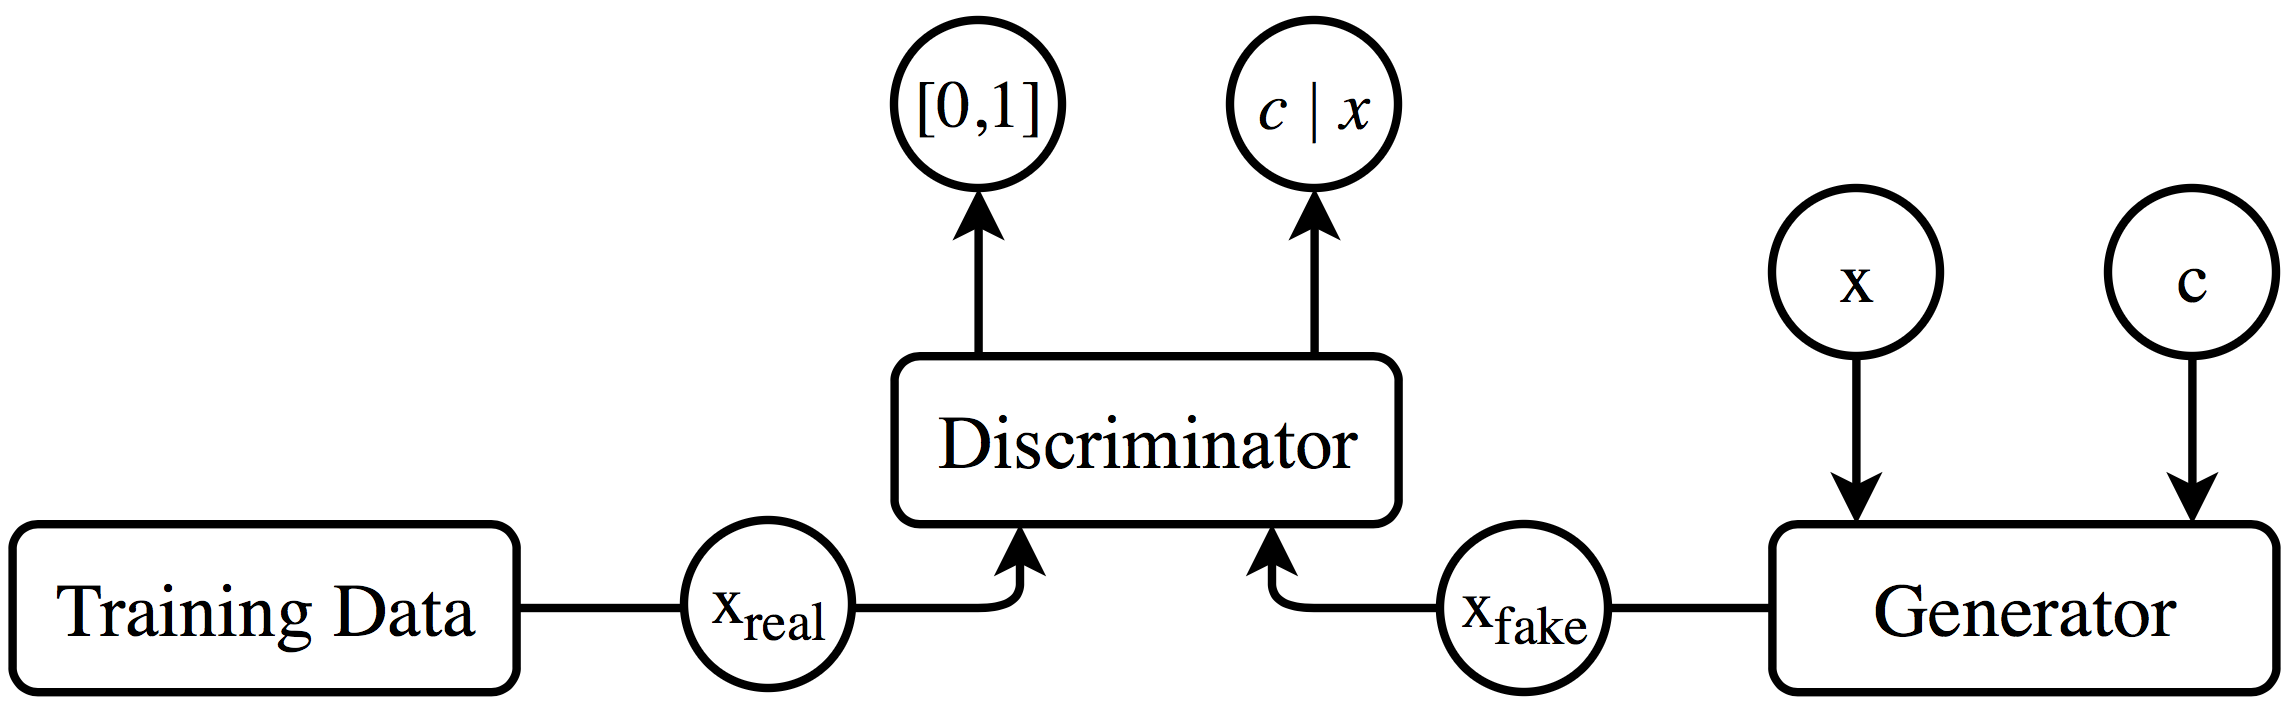
\includegraphics[width=3.5in]{pictures/diagram.png}
\caption{\textbf{Visual Representation of InfoGAN:} The Q network shares the same properties as the discriminator except it has one fully connected layer to output $Q(c|x)$.}  
\end{figure}

% Declare figure in previous page, so it can format to next page.

\begin{figure*}
    \centering
    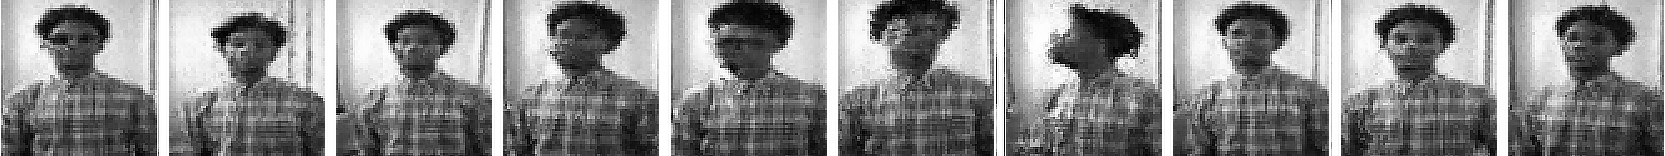
\includegraphics[width=7.25in]{pictures/personal/rasheed-flipped.jpg}\vspace*{2mm}
    \hspace*{.15mm}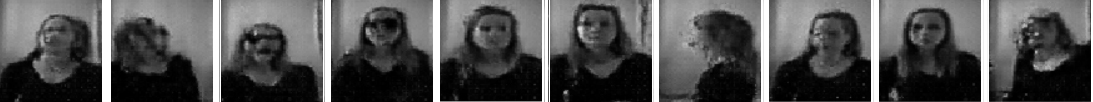
\includegraphics[width=7.25in]{pictures/personal/lilly-flipped.jpg}
    \caption{\textbf{Results from Personal Dataset:} When trained on a Categorical variable of dimension 2, the network independently generated images of both subjects, Rasheed and Lilly, to fill those two slots.}
\end{figure*}

\begin{figure*}
    \centering
    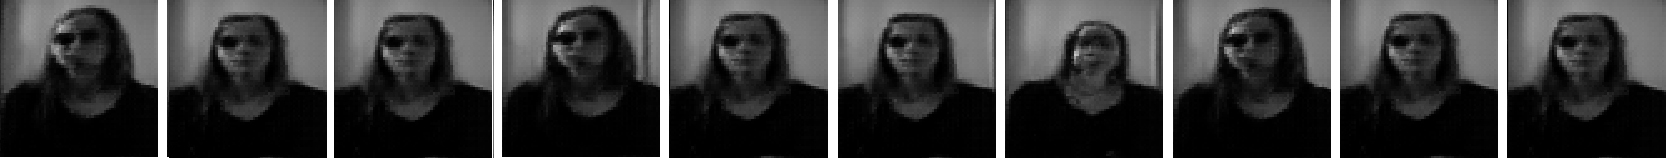
\includegraphics[width=7.25in]{pictures/personal/lilly-glasses-final.jpg}\vspace*{2mm}
    \hspace*{.15mm}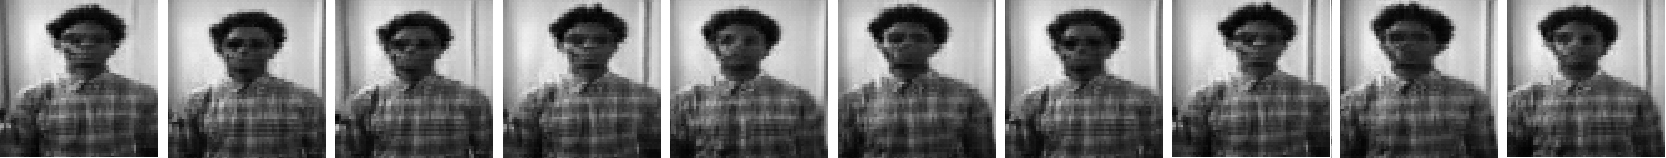
\includegraphics[width=7.25in]{pictures/personal/rasheed-glasses-final.jpg}
    \caption{\textbf{Results from Personal Dataset:} When trained on a Categorical variable of dimension 50, the network discovered glasses on a subject's face.  Notice the darker areas around the eyes.  In the training data, there were 175 photos of each subject wearing glasess.}  
\end{figure*}

% ** Politicians ** %
\begin{figure*}
    \centering
    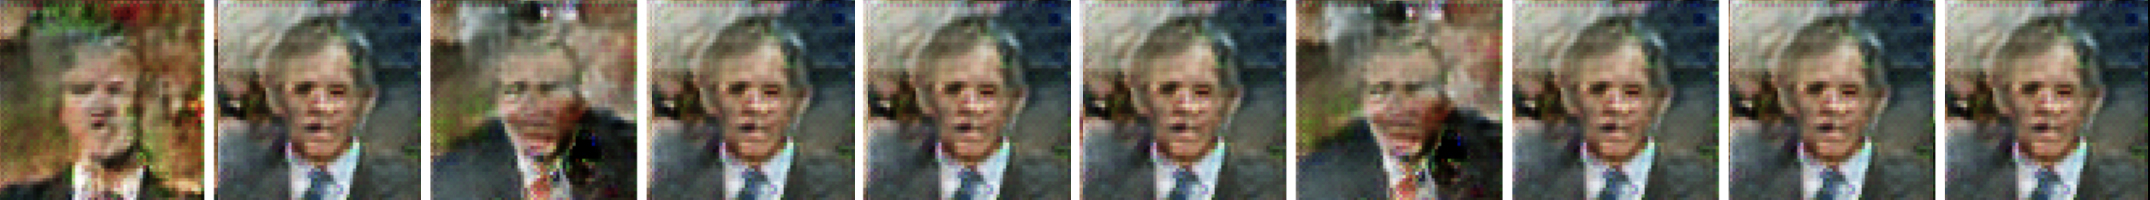
\includegraphics[width=7.25in]{pictures/politicians/bush-final.jpg}\vspace*{2mm}
    \hspace*{.15mm}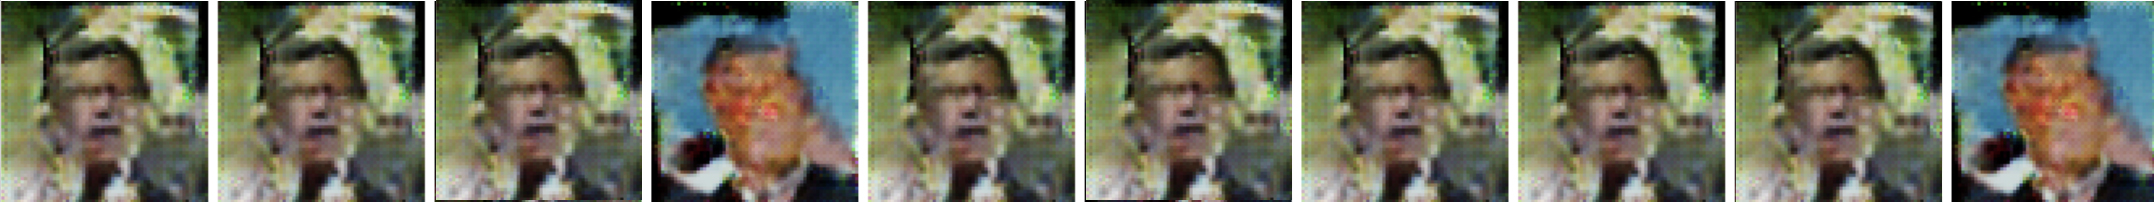
\includegraphics[width=7.25in]{pictures/politicians/schroeder-final.jpg}\vspace{2mm}
    \hspace*{.15mm}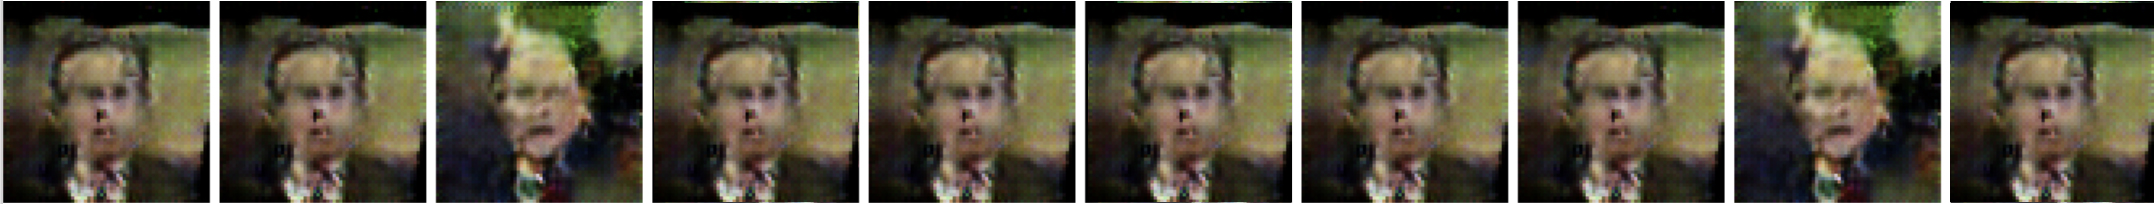
\includegraphics[width=7.25in]{pictures/politicians/blair-final.jpg}\vspace{2mm}
    \hspace*{.15mm}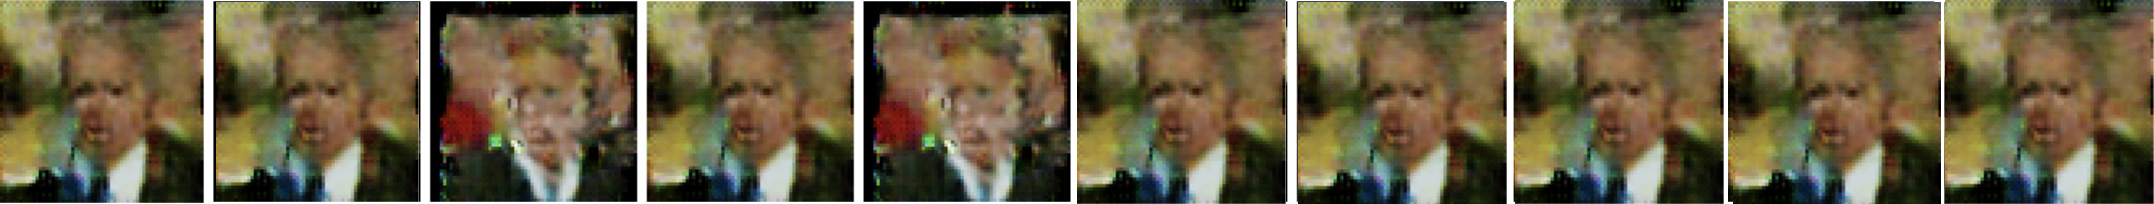
\includegraphics[width=7.25in]{pictures/politicians/powell-final.jpg}\vspace*{2mm}
    \hspace*{.15mm}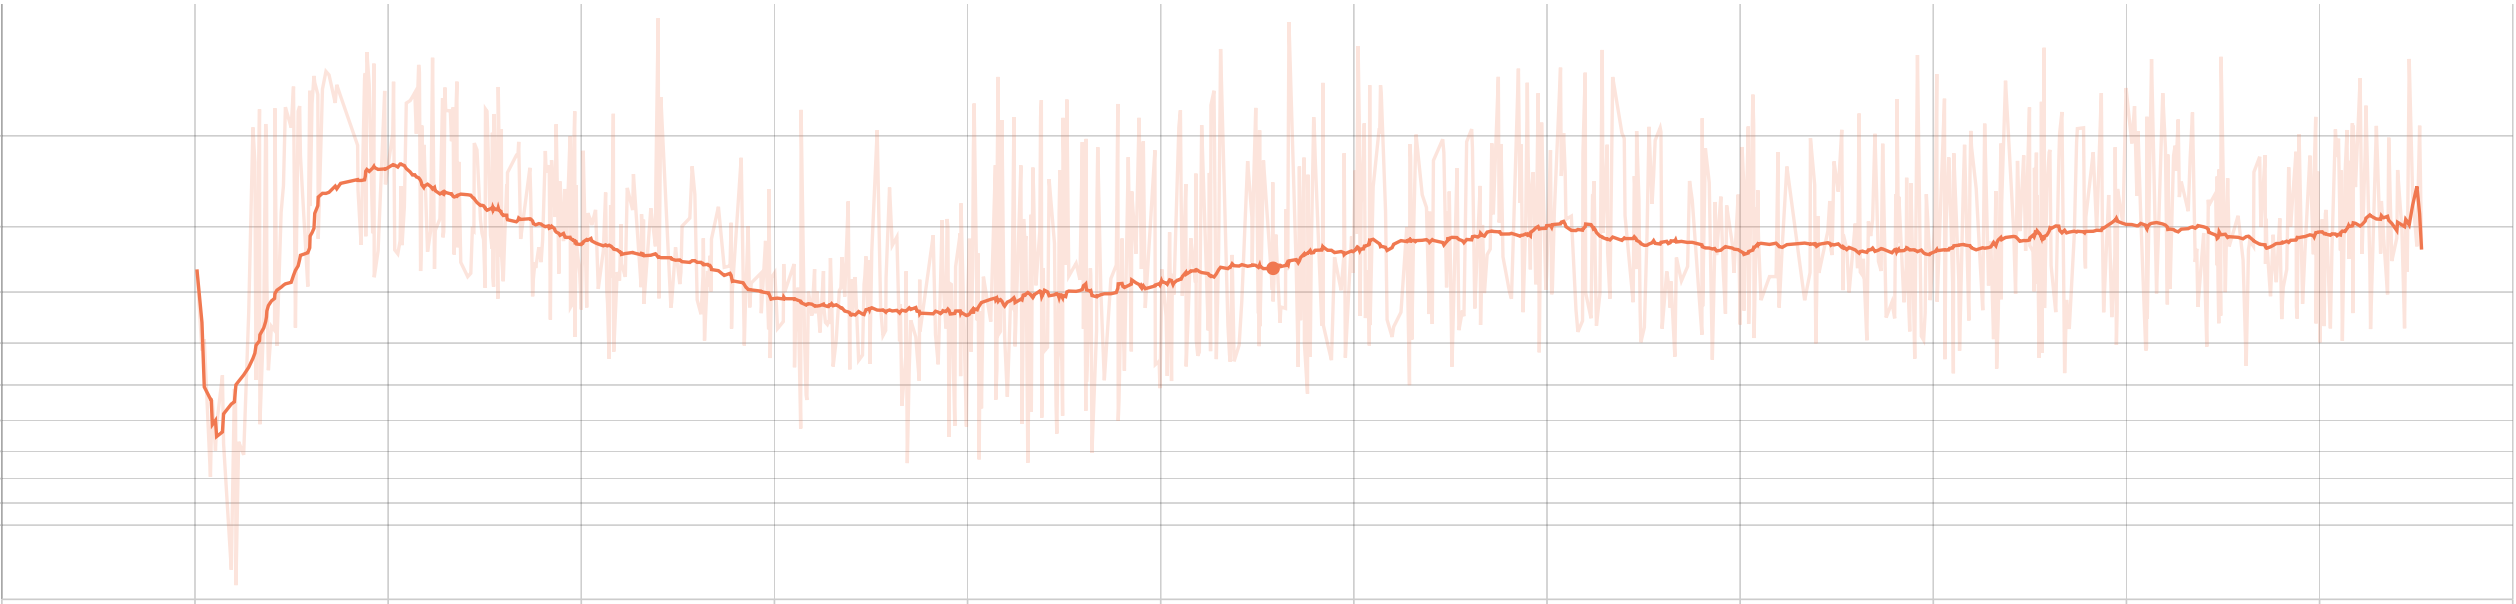
\includegraphics[width=7.25in,height=1in]{pictures/politicians/generatorOBJ.png}\vspace*{2mm}
    \hspace*{.15mm}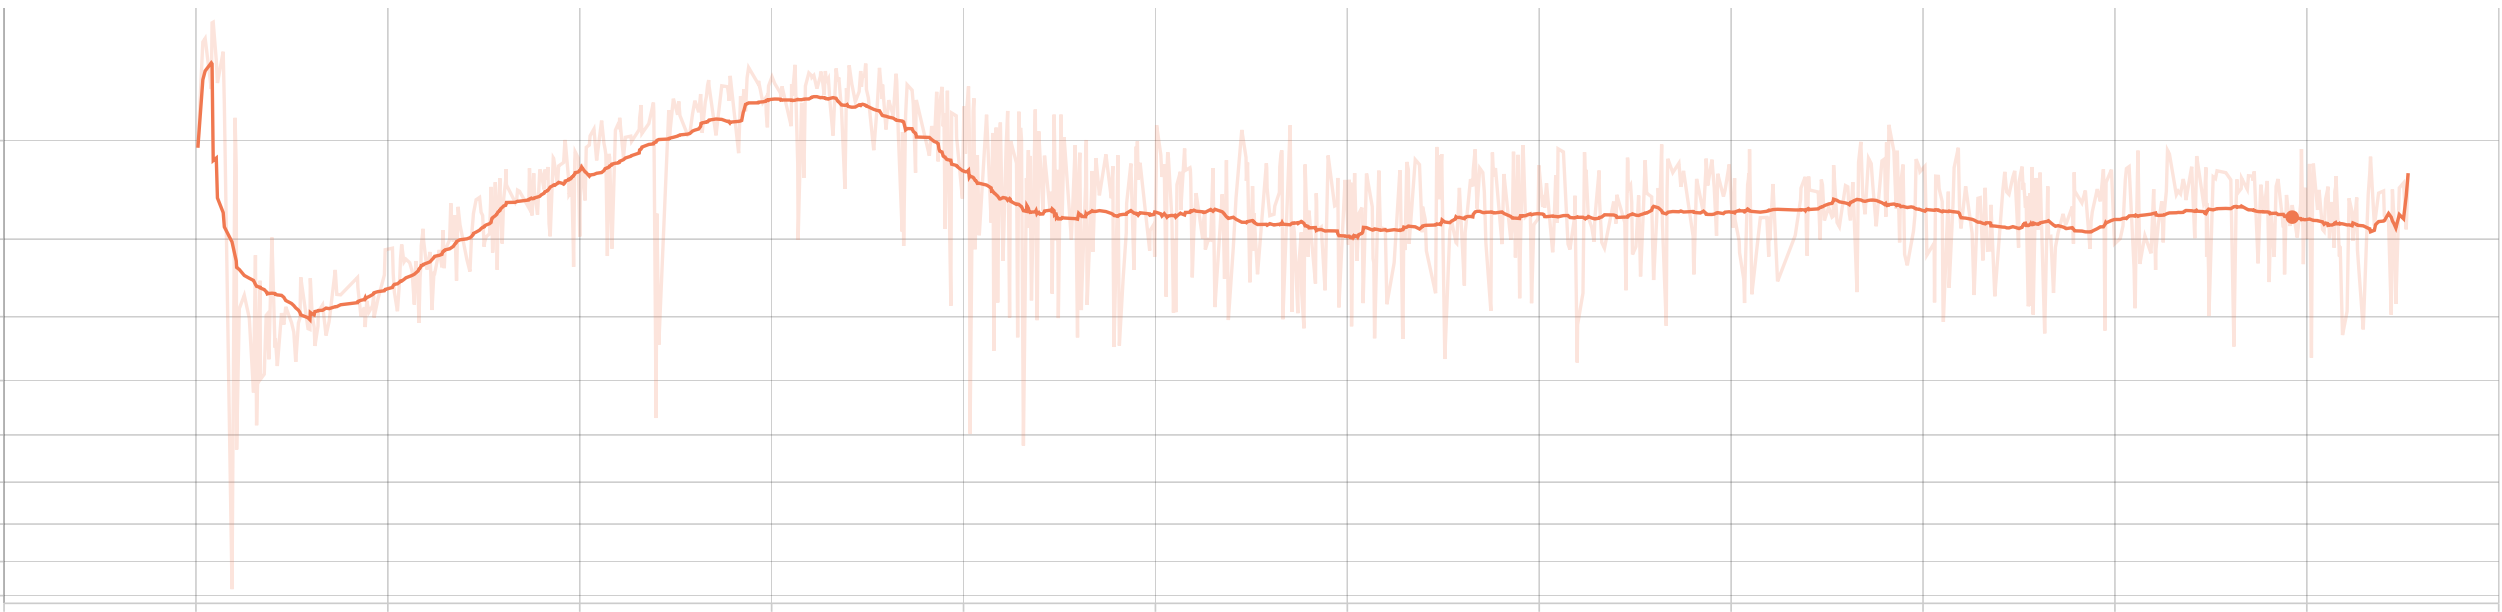
\includegraphics[width=7.25in,height=1in]{pictures/politicians/discriminatorOBJ.png}
    \caption{\textbf{Results from Politicians Dataset:} When trained on a Categorical variable of dimension 5, the network independently generated images of each politician, excluding Hugo Chavez.  From top to bottom, we have George W. Bush, Gerhard Schroeder, Tony Blair, and Colin Powell.  The fifth slot, not depicted, had images that contained of a mixture of all subjects.  Also shown are two plots of the network objectives.  The top graph is the generator and the bottom is the discriminator.}
\end{figure*}

This new variable, $c$, is the variable to which the network learns to fit the generated images.  We may specify several Categorical and Continuous variables as input and the Generator will fit increasingly realistic images to those variables.  However, since $c$ is a more generic version of $y$, we must train a third deep network, call it $Q$, which aims to approximate $c$, the latent code, given $x$, an element from the dataset.  $Q$ isn't explicitly a crafted as a third network because it shares all of the same features as the discriminator. So we can simplify the structure of the network sharing the layers of $D$ and $Q$,  only adjusting the final output layer of $Q$ to produce different results.  A model of network topology is shown in Figure 2.

Without $Q$, the generator could easily deteriorate back into $G(z)$, therefore, $Q$ aims to maximize the mutual information between $x$ and $c$.  In Information Theory, maximizing the two random variables X and Y, $I(X;Y)$, is defined as the difference in their entropies.  This also proposes a new value function:
\begin{equation}
    I(X;Y) = H(X) - H(X|Y) = H(Y) - H(Y|X)
\end{equation}
\begin{flalign}
\begin{split}
\minGAN_{G}\maxGAN_{D}V_1(D,G) = V(D,G) + \lambda I(c;G(z,c))
\end{split}
\end{flalign}

Because we want mutual information to be high, we aim to minimize $I(c;G(z,c))$, so we require the distribution of $P(c|x)$.  Luckily, the third network, $Q(c|x)$, gives an accurate approximation of the posterior $P(c|x)$.  $I(c;G(z,c))$ is computed and minimized using a lower bound maximization called Variational Information Maximization.  Finally, InfoGAN is defined as the following minimax game with a new value function, where $L_1$ is the variational lower bound:
\begin{flalign}
\begin{split}
\minGAN_{G}\maxGAN_{D}V_{\text{InfoGAN}}(D,G,Q) = V(D,G) - \lambda L_1(G,Q)
\end{split}
\end{flalign}


\section{Datasets}
In order to conduct unsupervised facial recognition with InfoGAN, we required a dataset with few individuals with many images per individual.  However, many online open sourced databases contained inconsistent images, having too many individuals.  In the few datasets found of single individuals, the images often had extremely high variance (full body vs. portrait) and included other people, text, or even borders. 

We created our own dataset: it consisted of only two people and captured those individuals in exclusively portrait photos, containing many different angles. During capture, the subjects would wear hats or sunglasses for a portion of the images. Technical description and sample images are provided in Appendix A.

In addition to this personal dataset, we trained the network on two others.  The first dataset, consisting of more than 900 images, contained photos of five politicians: George W. Bush, Gerhard Schroeder, Hugo Chavez, Colin Powell, and Tony Blair.  The second dataset, also containing roughly 900 photos, focused on drawings and paintings from Vincent Van Gogh and Rembrandt van Rijn.

% TODO RESUME HERE


\section{Experiments}

\subsection{Personal Dataset}

As hypothesized, when the network was trained on the personal dataset, which consisted of images from two subjects, it was able to successfully distinguish between both subjects.  In Figure 3, we see two sets of images that distinctly resemble both subjects.  InfoGAN learned a dimension-2 Categorical variable that fit one subject, Rasheed, to one dimension and the other suject, Lilly, to the other.

We additionally specified a Categorical of dimension 50 and pulled out two sets of images, shown in figure 4, where InfoGAN recognized sun glasses on a subject's face.  By recognizing facial accessories, InfoGAN relates to our larger hypothesis by drawing out other specific, relevant, high dimensional, features from the training data.  Additionally, it learned high dimensional characteristics, such as full body rotation, and assigned that to a continuous variable, as shown in Figure 1. Research has demonstrated that the motion of faces appear to facilitate recognition \cite{faceRecog}, and InfoGAN, by discovering rotation, supports that hypothesis.

\begin{table}[h]
\centering
\caption{Hyperparameters for Personal Dataset}
\resizebox{.35\textwidth}{!}{%
\begin{tabular}{|p{3cm}|p{3cm}|p{3cm}}
\hline
Epochs                         & \multicolumn{2}{l|}{10000}         \\ \hline
Continuous Variables           & \multicolumn{2}{l|}{2}             \\ \hline
Categorical Cardinality        & \multicolumn{2}{l|}{2, 5, 10, 20}  \\ \hline
Categorical Lambda             & \multicolumn{2}{l|}{1}             \\ \hline
Continuous Lambda              & \multicolumn{2}{l|}{1}             \\ \hline
\end{tabular}%
}
\end{table}


\begin{figure*}[ht]
    \centering
    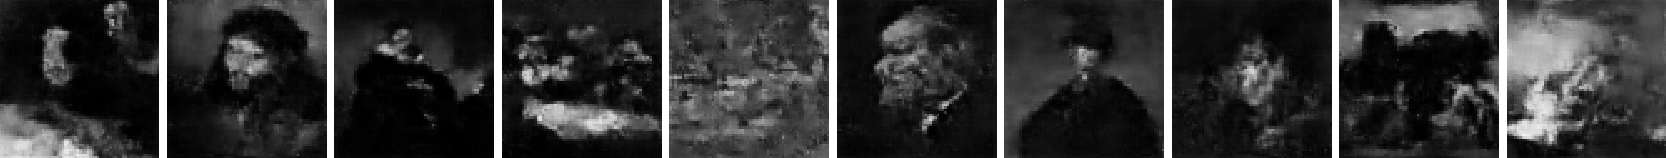
\includegraphics[width=7.25in]{pictures/Datasets/art/betterRembrandt_dim2.jpg}\vspace*{2mm}
    \hspace*{.15mm}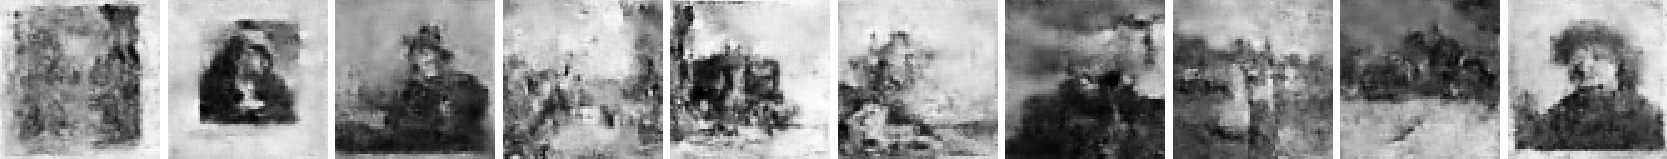
\includegraphics[width=7.25in]{pictures/Datasets/art/betterVanGogh_dim2.jpg}
    \caption{\textbf{Paintings Dataset: Author classification:} When trained on a Categorical variable of dimension 2, the network independently generated images closely resembling artwork produced by Rembrandt van Rijn (top sequence) and Vincent Van Gogh (bottom sequence).}
\end{figure*}

\begin{figure*}[ht]
    \centering
    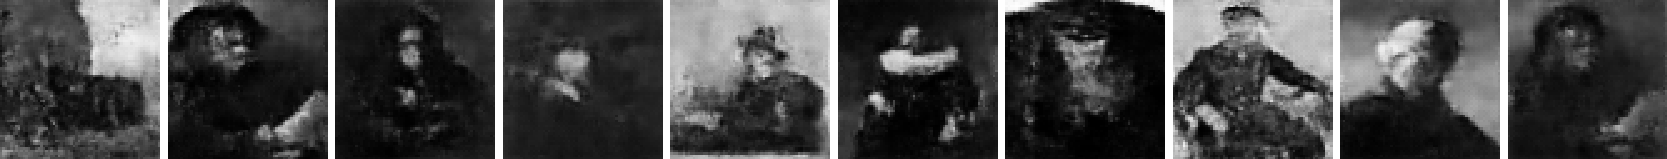
\includegraphics[width=7.25in]{pictures/Datasets/art/great_rembrandt_portraits.jpg}\vspace*{2mm}
    \hspace*{.15mm}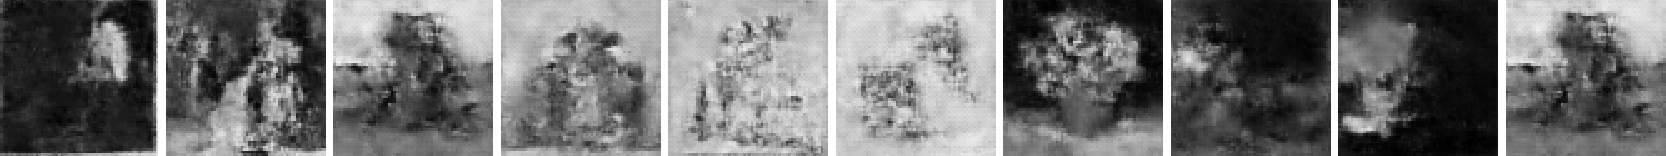
\includegraphics[width=7.25in]{pictures/Datasets/art/VanGogh_flowers.jpg}
    \caption{\textbf{Paintings Dataset Subject Capture:} A categorical variable of dimension 20 was trained in order to capture the many different styles and subjects that each author painted.  The top images are exclusively mid-body portraits painted by Rembrandt.  The bottom image is less clear, but are of flowers painted by Van Gogh.}
\end{figure*}

%\begin{figure*}[ht]
%\centering
%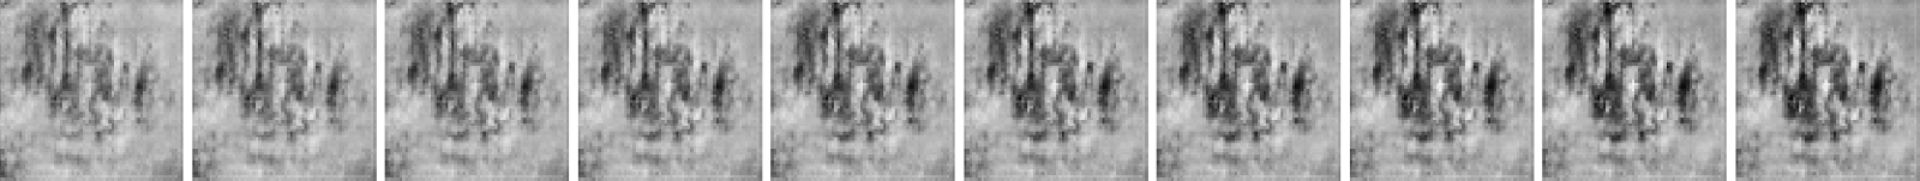
\includegraphics[width=7.25in]{pictures/Datasets/art/continuousLineThicc.png}\vspace*{2mm}
%\hspace*{.15mm}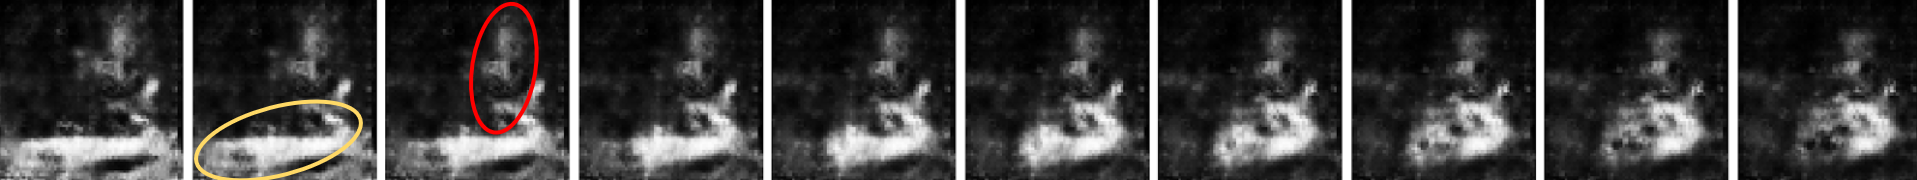
\includegraphics[width=7.25in]{pictures/Datasets/art/contStyleCircled.png}
%\caption{\textbf{Paintings Dataset Style Capture:} A Categorical variable of dimension 20 was trained in order to capture the many different styles and subjects that each author painted.  The top images are exclusively mid-body portraits painted by Rembrandt.  The bottom image is less clear, but are of flowers painted by Van Gogh.  The quality of flowers are lower because there are only 18 flower images in the Van Gogh dataset.}
%\end{figure*}

\subsection{Politicians}

When InfoGAN was trained on a dataset containing five politicians, it was able to successfully discern between four of the five subjects, but failed on the subject with by far the fewest training examples.  In Figure 5, each set of images are distinct from the other, clearly depicting different individuals from the training data.  InfoGAN exceeded our expectations from the personal dataset, where we only predicted it would be able to tell apart two subjects.

However, we note that the fifth politician, Hugo Chavez, is missing.  We assume this is largely due to the lack of available training data.  The Chavez dataset only contained roughly 70 images, whereas the dataset contained roughly 100-500 images each of the other four politicians.  Therefore, the results are heavily skewed toward individuals with a higher amount of images.

Also shown in figure 5 are the generator and discriminator objectives.  These serve as quantitative ways to measure the progress and functionality of our network.  Logically, both networks should have an inverse relationship, since the generator increasingly produces realistic images while the discriminator struggles to discern between the two sets.  The graphs demonstrate this fact: the generator begins with an upward trend and the discriminator down.  Both networks steadily rise and fall with time before converging to a straight line.  The generator and discriminator converged to a straight line at around epoch 6500, at which point they reached Nash Equilibrium.   The input parameters for the politician results are shown in table 2.

For the discriminator's objective, the plot shows the desired loss function.  Recall that we want to maximize $D$'s objective function, $\log D(x) + \log (1-D(G(z)))$. The desired value of this function is 0.5, which implies that the discriminator won't be able to distinguish between the real and fake data.  In the discriminator's plot, the graph converges to a value of 0.5 though the axis labels aren't shown.  The plots empiracally show the accuracy of our networks and provide further proof that the generated data matches our predictions.

\begin{table}[h]
\centering
\caption{Hyperparameters for Politician Dataset}
\resizebox{.35\textwidth}{!}{%
\begin{tabular}{|p{3cm}|p{3cm}|p{3cm}}
\hline
Epochs                         & \multicolumn{2}{l|}{10000} \\ \hline
Continuous Variables           & \multicolumn{2}{l|}{3}     \\ \hline
Categorical Cardinality        & \multicolumn{2}{l|}{5, 2}  \\ \hline
Categorical Lambda             & \multicolumn{2}{l|}{0.5}   \\ \hline
Continuous Lambda              & \multicolumn{2}{l|}{0.5}   \\ \hline
\end{tabular}%
}
\end{table}

\subsection{Art: Paintings of Picasso and Rembrandt}

InfoGAN, when trained on a relatively complex art dataset, discerned between the distinct styles and subjects of both artists.  Moreover, due to the generative nature of InfoGAN, it captured representations of their artistic techniques and exposed those motifs to the viewer, thereby aiding a user in understanding the artists.  InfoGAN learned representations of both artists's style when given a categorical variable of dimension 2.  Notably, both variables come close to expressing the full range of the authors' work, as opposed to a single style.  The network learned the overarching nature of an artist's style and content, based on many sample images.  Figure 6 depicts our result: the top set of generated image resembles Rembrandt's darker, harder, more outlined figures.  The bottom set portrays Van Gogh's landscapes and portraitures as well as his softer, and less defined brush strokes. 

When given a Categorical variable of dimension 20, InfoGAN learned specific categories of work from each artist.  In Figure 7, the top set features exclusively mid-body portraits, which closely match Rembrandt's style in the dataset.  The bottom set, though harder to observe, depict flowers, which are a key object in Van Gogh's artwork.  The lower quality of the flowers occur because there are only 18 images of flowers in the Van Gogh dataset.  Figure 7, however, only depicts two out of the available 20 dimensions of the specified categorical variable.  Many different categories were captured, but overlap or between variables is also somewhat common.

\begin{table}[h]
\centering
\caption{Hyperparameters for Art Dataset}
\resizebox{.35\textwidth}{!}{%
\begin{tabular}{|p{3cm}|p{3cm}|p{3cm}}
\hline
Epochs                         & \multicolumn{2}{l|}{5000} \\ \hline
Continuous Variables           & \multicolumn{2}{l|}{2}     \\ \hline
Categorical Cardinality        & \multicolumn{2}{l|}{2, 20, 50}  \\ \hline
Categorical Lambda             & \multicolumn{2}{l|}{1}   \\ \hline
Continuous Lambda              & \multicolumn{2}{l|}{1}   \\ \hline
\end{tabular}%
}
\end{table}

\section{Discussion}

During the training of the network, we want to discuss three important aspects of how our network functioned. The first is the number of epochs specified.  In tables 1, 2, and 3, we list the number of epochs for which each network was trained. These were chosen to prevent overfitting. Originally, we believed that more epochs, which provides more training time, would aid the generator, since our datasets offered limited amounts of training data.  However, as seen in the graphs of Figure 5, exemplifying longer, over-fit round of training, the two networks' objective flattened about midway through, which prompted us to limit our amount of training to around that value of convergence.  We discovered that if the network overtrained, the generator would produce images that has no resemblance to the original dataset, or where each latent code represented identical properties from the data.

Following our original belief that fewer images require fewer epochs, the quality of an individual image depends on the amount of training examples in the dataset.  As opposed to the original InfoGAN paper, which tested the network on the CelebA and MNIST dataset, containing over 200,000 images each, we were limited by publicly available material.  The politician and art datasets only had at maximum 500 images per subject (each with 950 images in total).  Hence, we opted to create our own dataset, with 2,500 photos each of two subjects.  These numbers are still far less than CelebA and MNIST, but InfoGAN still produced recognizable images, despite the lower quality and grainy features.  Additionally, the training time per epoch scales with the number of images and its resolution: the CelebA dataset takes approximately 14 minutes/epoch, and our personal dataset around 20 seconds/epoch in Tensorflow on a Nvidia GTX 1080 graphics card.  In order to demonstrate the striking difference in quality, we trained our network on the CelebA dataset and compare those images with our personal set in Figure 8.

\begin{figure}[ht]
    \centering
    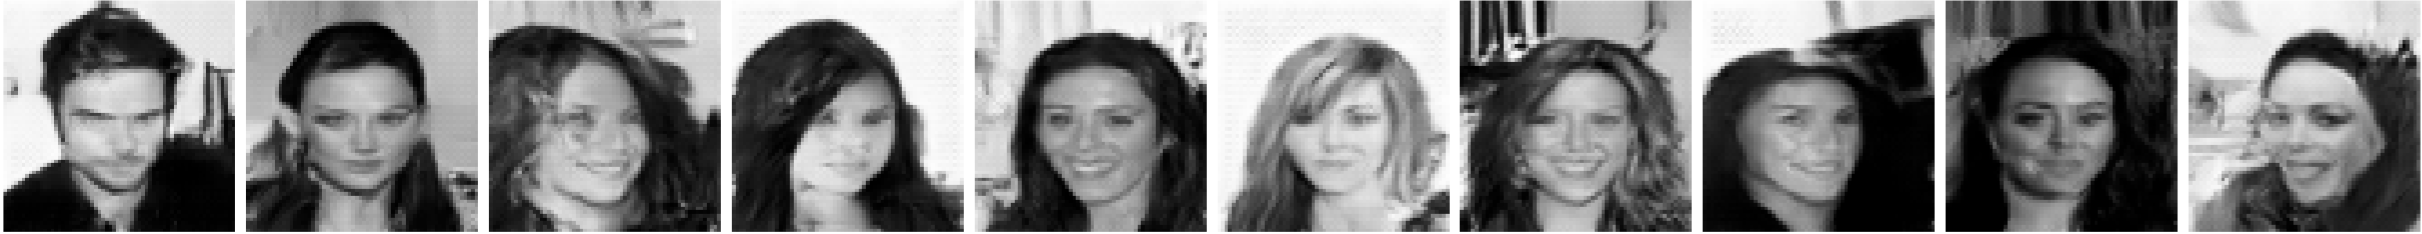
\includegraphics[width=\linewidth]{pictures/celeba1.png}
    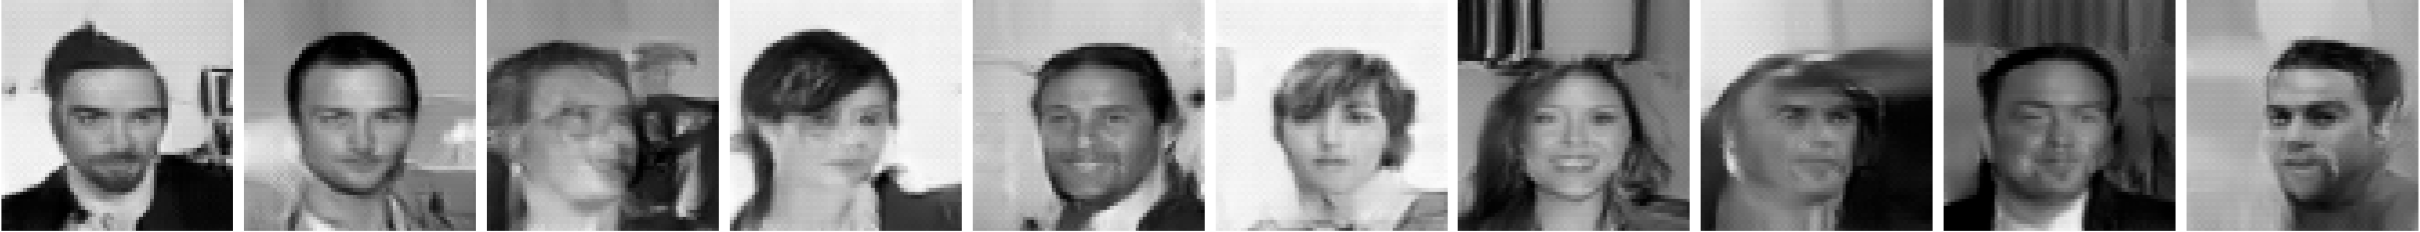
\includegraphics[width=\linewidth]{pictures/celeba2.png}\vspace{2mm}
    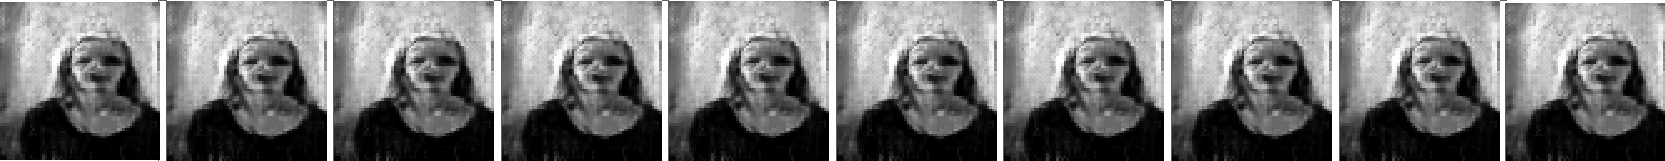
\includegraphics[width=\linewidth]{pictures/personal/lilly-ahead-final.jpg}
    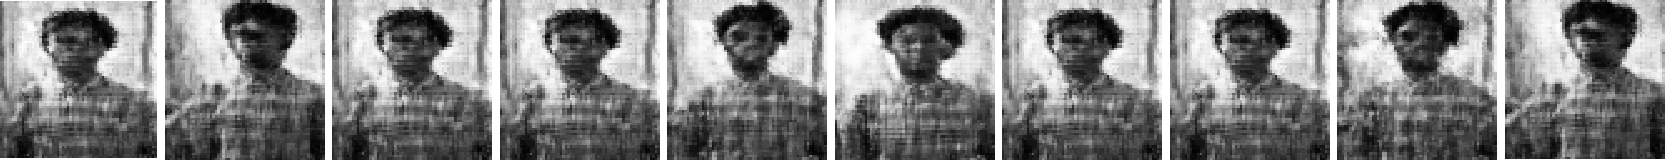
\includegraphics[width=\linewidth]{pictures/personal/rasheed-ahead-final.jpg}   
    \caption{\textbf{Comparision of Quality:} The top two rows of images were taken from the CelebA dataset.  The bottom to rows are taken from the personal dataset.}
\end{figure}

A limitation of our research was not only time, but an intrinsic property of images that most take for granted: color.  Our results from the art and personal dataset contained images where we forced the network to generate grayscale.  Colored images are created with several stacked color channels, namely red, green, and blue (RGB).  Grayscale images only contain one alpha channel, where each pixel value represents the intensity of light.  When training InfoGAN, we must manipulate our network in such a way that it can accept grayscale or RGB images.  This changes how the  discriminator can process images.  With extensive testing, we conclude that the network has a difficult time parsing through images of three channels, as opposed to one.  This increases the time complexity of the algorithm, forcing every epoch to take roughly 3 times as long.

When generating images of color, the art dataset had a difficult time training the latent codes.  We obtained images which somewhat resembled the subjects, but they were mostly a block of colors.  However, the politician dataset, produced had exemplary results: the subjects are clear and distinct from one another.  We believe this is largely due to the obvious differences between a real photo and a painting.  With larger datasets that can equally match the size of CelebA, we predict that InfoGAN would be able to support our results with color, if given the appropriate parameters. 

\section{Conclusion}

InfoGAN successfully discerned among two, and even five, individuals in the given training dataset.  It also learned key discrete and continuous features of the subjects like the presence of glasses and their rotation.  The network additionally captured Van Gogh's and Rembrandt's artistic subjects and styles, generating sets of images that portray each artist's painting technique.  Their overarching styles were accurately captured in a dimension-2 categorical variable, while their specific subjects and individual motifs were captured in larger dimension variables.  Continuous properties like brush stroke thickness, and lighting motifs were also captured and exposed to the viewer in continuous variables. 

Despite the lack of color in two of our experiments, our results are fascinating because it presents a window where we may possibly understand how humans recognize objects and perform recognition.  Learning these traits and styles in a completely unsupervised manner gives insight into the possibilities of future research, which include successfully generating colored images, expanding the personal dataset with more examples, and performing finer tuning of the Categorical or Continuous variables and learning rates.

% use section* for acknowledgement
\section*{Acknowledgment}

The authors would like to thank the authors of the original InfoGAN paper, and OpenAI for sponsoring their research and making it available to the open source community. We would also like to thank the many groups which made their data available online such as the University of Massachusetts Amherst, the Web Gallery of Art, and friends Lilly and Rasheed for posing for thousands of photos.  We would also like to thank Professor Lisa Meeden for her guidance during this project. 

\ifCLASSOPTIONcaptionsoff
  \newpage
\fi

% references section
\bibliographystyle{IEEEtran}
\bibliography{ref.bib}{}

\appendices
\section{Personal Dataset}

%Table describing dataset:
\begin{table}[ht]
\caption{Personal Dataset Contents}
\centering
    \begin{tabular}{ |p{4cm}||p{1.5cm}|p{1.5cm}|p{3cm}|  }
     \hline
        & Lilly &Rasheed\\
     \hline
     Normal \& Angled & 1600    &1600\\
     Sunglasses& 725 & 725 \\
     Sunglasses on Head & 175 & 175\\
     \hline
     Total    &2500 & 2500\\
     \hline
    \end{tabular}
\end{table}

\begin{figure}[ht]
    \centering
    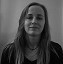
\includegraphics[width=1in]{pictures/Datasets/64pixStraightSquareBW.jpg}
    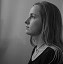
\includegraphics[width=1in]{pictures/Datasets/64pix45degSquareBW.jpg}
    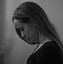
\includegraphics[width=1in]{pictures/Datasets/64pix90degSquareBW.jpg}
    \caption{\textbf{Sample Normal Images of Lilly:} Example `Normal \& Angled' images. Angled images were captured in both directions, and with the subject's head at many different vertical and rotational angles.}
\end{figure}

\begin{figure}[ht]
    \centering
    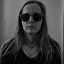
\includegraphics[width=.82in]{pictures/Datasets/glassesStraight.jpg}
    
\includegraphics[width=.82in]{pictures/Datasets/GlassesForheadStraight.jpg}
    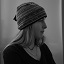
\includegraphics[width=.82in]{pictures/Datasets/Hat90deg.jpg}
    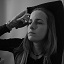
\includegraphics[width=.82in]{pictures/Datasets/armsUp.jpg}
    \caption{\textbf{Sample Feature Images of Lilly:} These images exemplify the 4 feature categories.  Wearing sunglasses, wearing sunglasses on forehead, wearing a cap, and arms above her head.}
\end{figure}

\begin{figure}[ht]
    \centering
    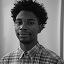
\includegraphics[width=1in]{pictures/rasheed/normalStraight.jpg}
    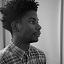
\includegraphics[width=1in]{pictures/rasheed/45deg.jpg}
    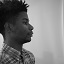
\includegraphics[width=1in]{pictures/rasheed/90deg.jpg}
    \caption{\textbf{Sample Normal Images from Rasheed:} Example `normal \& angled' images from Rasheed. Angled images were captured in both directions, and with the subject's head at many different vertical and rotational angles.}
\end{figure}

\begin{figure}[H]
    \centering
    
\includegraphics[width=1in]{pictures/rasheed/sunGlasses.jpg}
    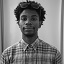
\includegraphics[width=1in]{pictures/rasheed/glassesUp.jpg}
    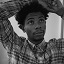
\includegraphics[width=1in]{pictures/rasheed/armsUp.jpg}
    \caption{\textbf{Sample Feature Images from Rasheed:} These images exemplify the 3 feature categories demonstrated by Rasheed.  Wearing sunglasses, wearing sunglasses propped on the his forehead and holding his arms above his head. Rasheed was not photographed wearing a hat, and therefore that feature was not compared in the combined facial recognition dataset.}
\end{figure}

This experiment found that altering the learning (lambda values) between 0.1 and 10 produced the best learned representations depending on the dataset and number of variables provided. In datasets with high-dimensional data, many more variables were required in order to provide adequate separation between learned traits. Higher dimensional variables are able to learn representations of each individual disentangled representation, whereas low dimensional variables will attempt to capture too many attributes into a single variable, leading to entangled representations and poorer results on complex data.  The following two tables, 5 and 6, show different parameters we tried during testing that gave accurate results. 

% Categorical hyperparemeters
\begin{table}[h]
\centering
\caption{Hyperparameters for Facial Recognition - Categorical Results}
\resizebox{.35\textwidth}{!}{%
\begin{tabular}{|p{3cm}|p{3cm}|p{3cm}}
\hline
Epochs                         & \multicolumn{2}{l|}{2000} \\ \hline
Continuous Variables           & \multicolumn{2}{l|}{2}     \\ \hline
Categorical Cardinality        & \multicolumn{2}{l|}{2, 20, 50}  \\ \hline
Categorical Lambda             & \multicolumn{2}{l|}{1}   \\ \hline
Continuous Lambda              & \multicolumn{2}{l|}{1}   \\ \hline
\end{tabular}%
}
\end{table}

% continuous hyperparemeters
\begin{table}[h]
\centering
\caption{Hyperparameters for Facial Recognition - Continuous Results}
\resizebox{.35\textwidth}{!}{%
\begin{tabular}{|p{3cm}|p{3cm}|p{3cm}}
\hline
Epochs                         & \multicolumn{2}{l|}{2000} \\ \hline
Continuous Variables           & \multicolumn{2}{l|}{5}     \\ \hline
Categorical Cardinality        & \multicolumn{2}{l|}{2}  \\ \hline
Categorical Lambda             & \multicolumn{2}{l|}{7}   \\ \hline
Continuous Lambda              & \multicolumn{2}{l|}{7}   \\ \hline
\end{tabular}
}
\end{table}

\section{Politicians Dataset}
This dataset of politicians was provided to the open source community by the University of Massachusetts Amherst under the name Labeled Faces in the Wild.  All images used in this study come from their most unedited collection, as opposed to alternatives which were aligned with 'deep funneling' as described on their website: http://vis-www.cs.umass.edu/lfw/.

%Table describing politicians:
\begin{table}[H]
    \caption{Politician Dataset Contents}
    \centering
    \begin{tabular}{ |p{1cm}||p{.8cm}|p{1cm}|p{1cm}| p{1.3cm}| p{.9cm}|}
        \hline
            &Bush &Powell &Blair &Schroeder &Chavez \\
        \hline
        Total & 530 &236 &144 &109 &71\\
        \hline
    \end{tabular}
\end{table}

\vspace{-1.5em}
\begin{figure}[ht]
    \centering
    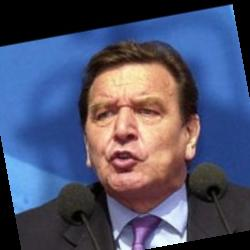
\includegraphics[width=1in]{pictures/politicians/schroeder-sample.jpg}
    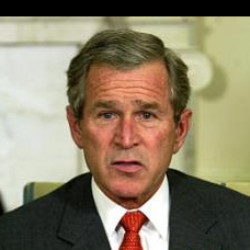
\includegraphics[width=1in]{pictures/politicians/bush-sample.jpg}
    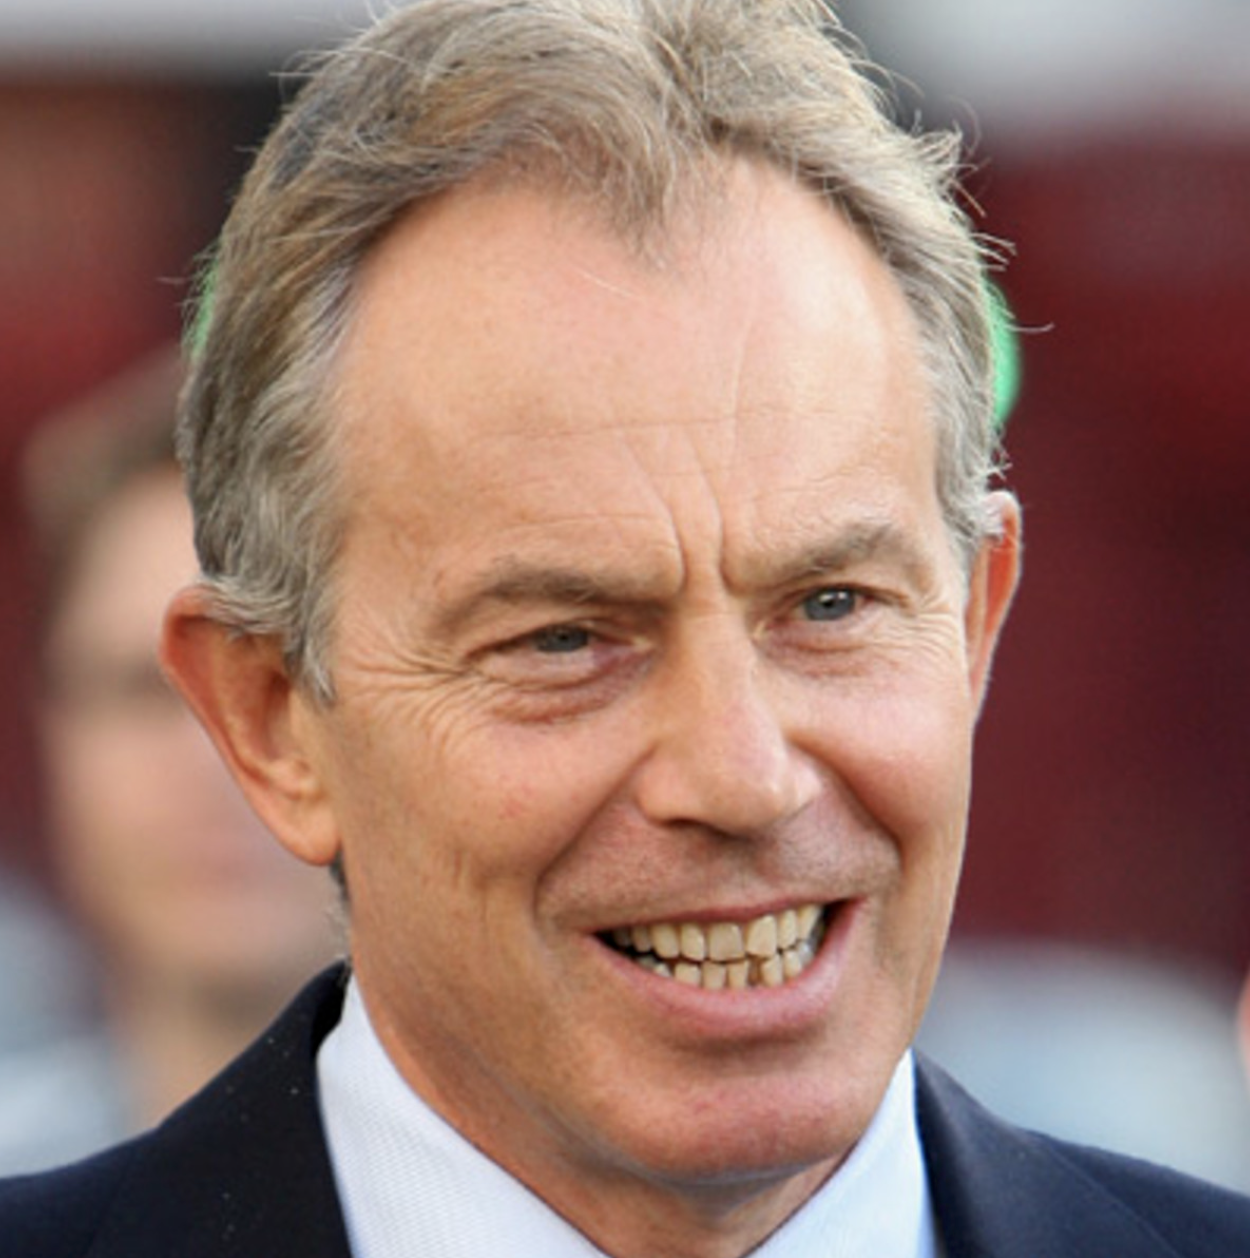
\includegraphics[width=1in]{pictures/politicians/blair-sample.png}
    \caption{\textbf{Sample Images of Politicians:} Example images from the Politician dataset.  Depicted from left to right are Gerhard Schroeder, George W. Bush, and Tony Blair}
\end{figure}

\section{Art Dataset}
The Art database consisted of 418 paintings from Vincent Van Gogh and 536 paintings from Rembrandt van Rijn.  The data was collected from the Web Gallary of Art (www.WGA.hu).  These two artists were chosen because of the volume of their work, and relatively different styles and subjects.

\begin{table}[H]
\centering
\caption{Hyperparameters for Art Dataset - Continuous Results}
\resizebox{.35\textwidth}{!}{%
\begin{tabular}{|p{3cm}|p{3cm}|p{3cm}}
\hline
Epochs                         & \multicolumn{2}{l|}{3600} \\ \hline
Continuous Variables           & \multicolumn{2}{l|}{2}     \\ \hline
Categorical Cardinality        & \multicolumn{2}{l|}{2, 20, 30}  \\ \hline
Categorical Lambda             & \multicolumn{2}{l|}{1}   \\ \hline
Continuous Lambda              & \multicolumn{2}{l|}{1}   \\ \hline
\end{tabular}
}
\end{table}

\begin{figure}[H]
    \centering
    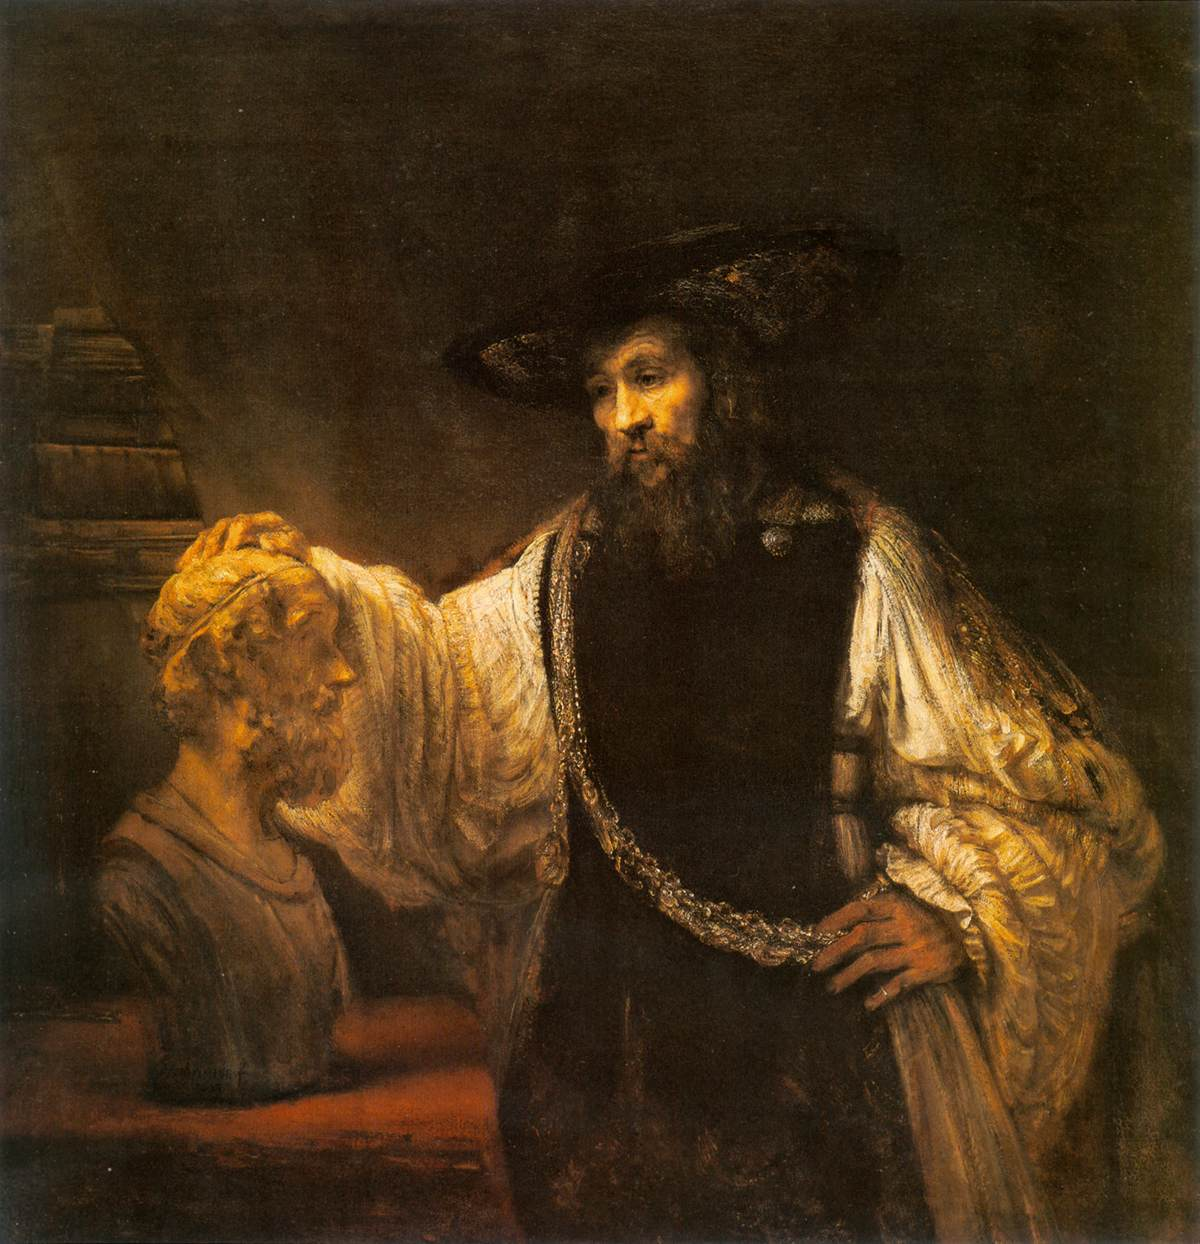
\includegraphics[width=.5in, height=.7in]{pictures/Datasets/art/rembrandt/Gogh109.jpg}
    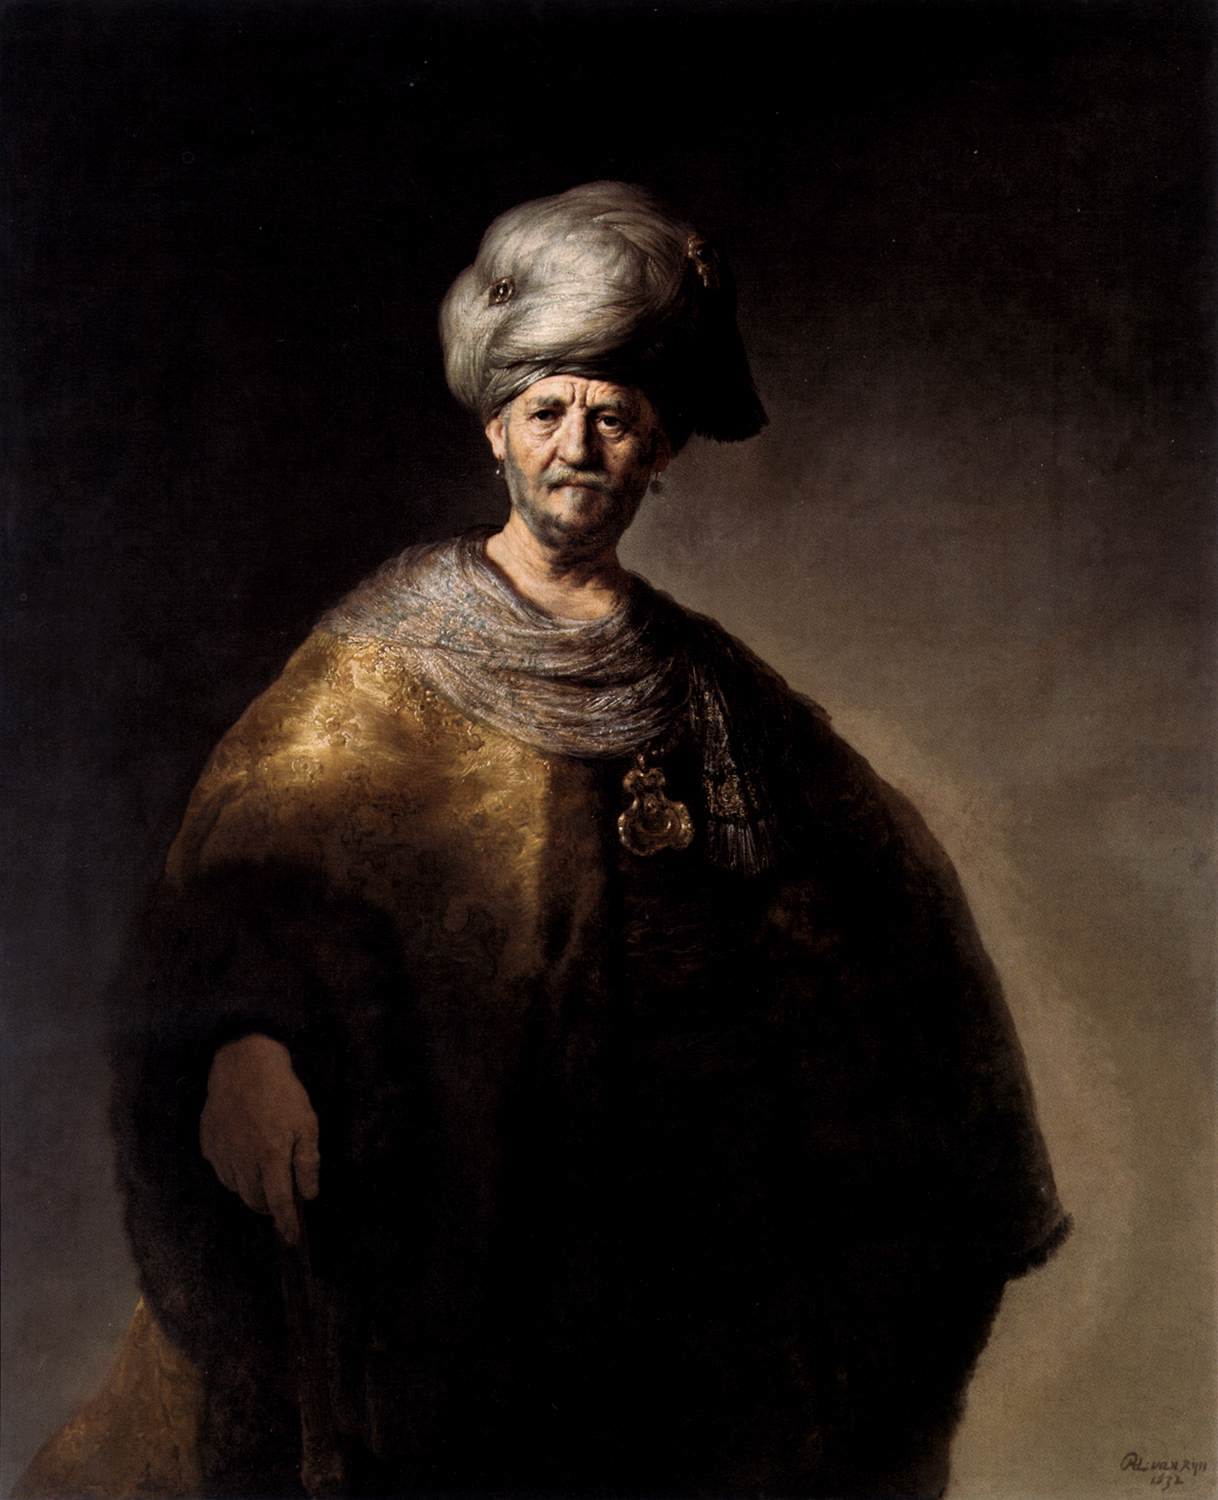
\includegraphics[width=.5in, height=.7in]{pictures/Datasets/art/rembrandt/Gogh131.jpg}
    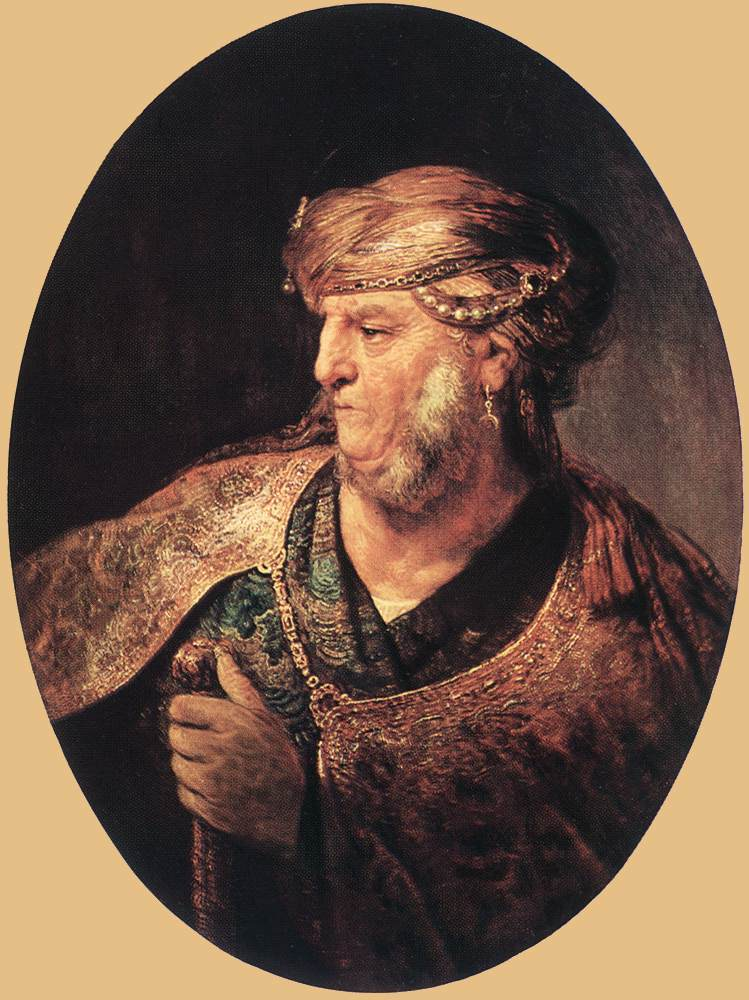
\includegraphics[width=.5in, height=.7in]{pictures/Datasets/art/rembrandt/Gogh148.jpg}
    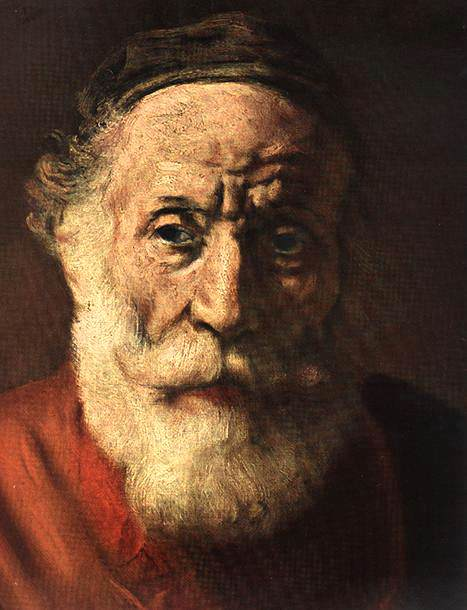
\includegraphics[width=.5in, height=.7in]{pictures/Datasets/art/rembrandt/Gogh181.jpg}
    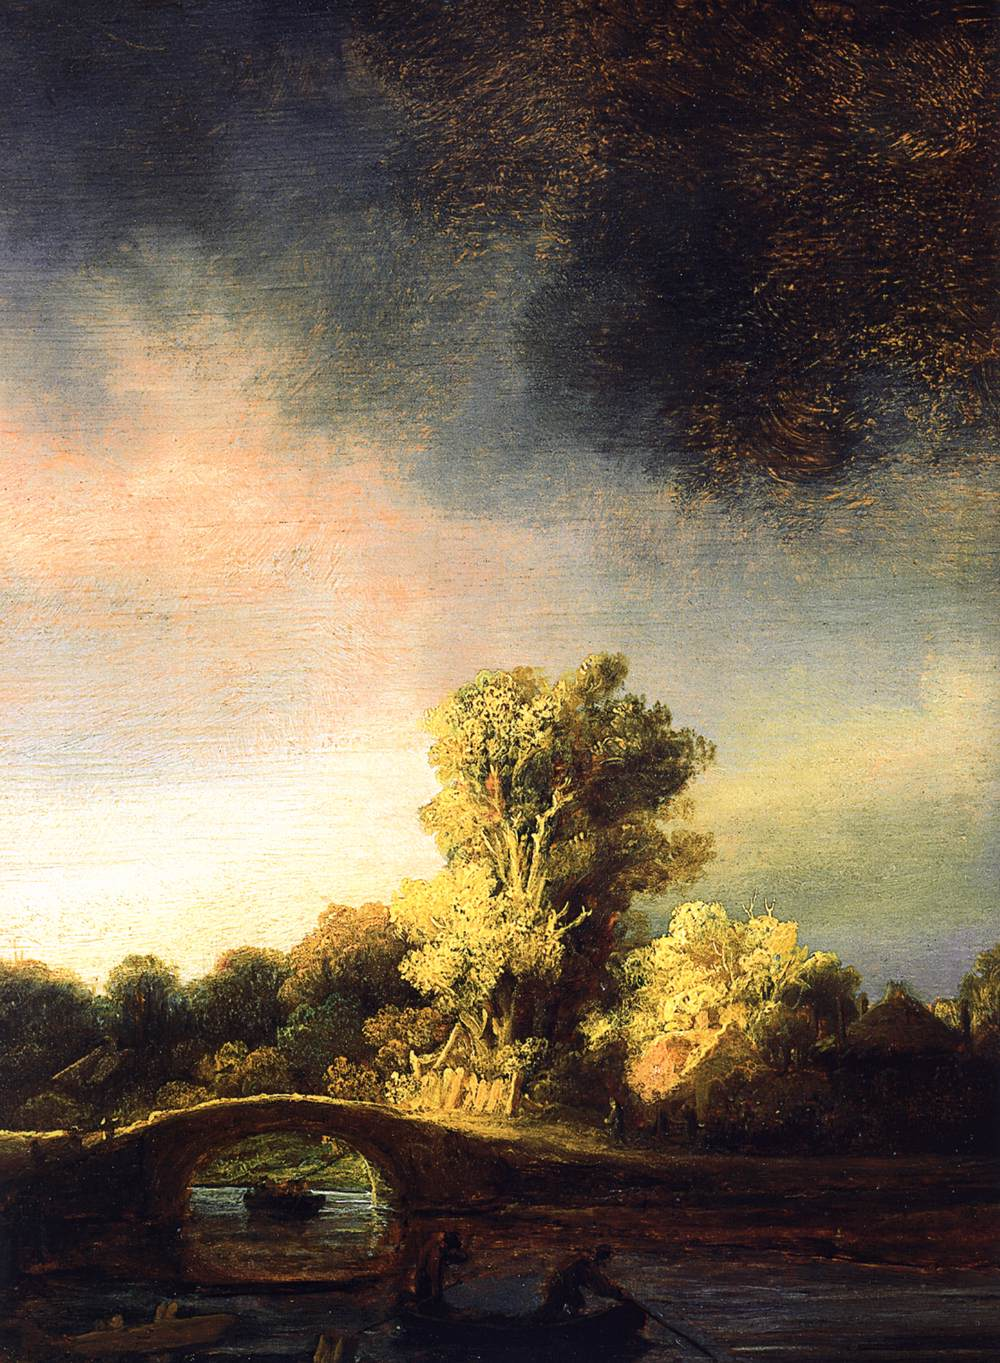
\includegraphics[width=.5in, height=.7in]{pictures/Datasets/art/rembrandt/Gogh267.jpg}
    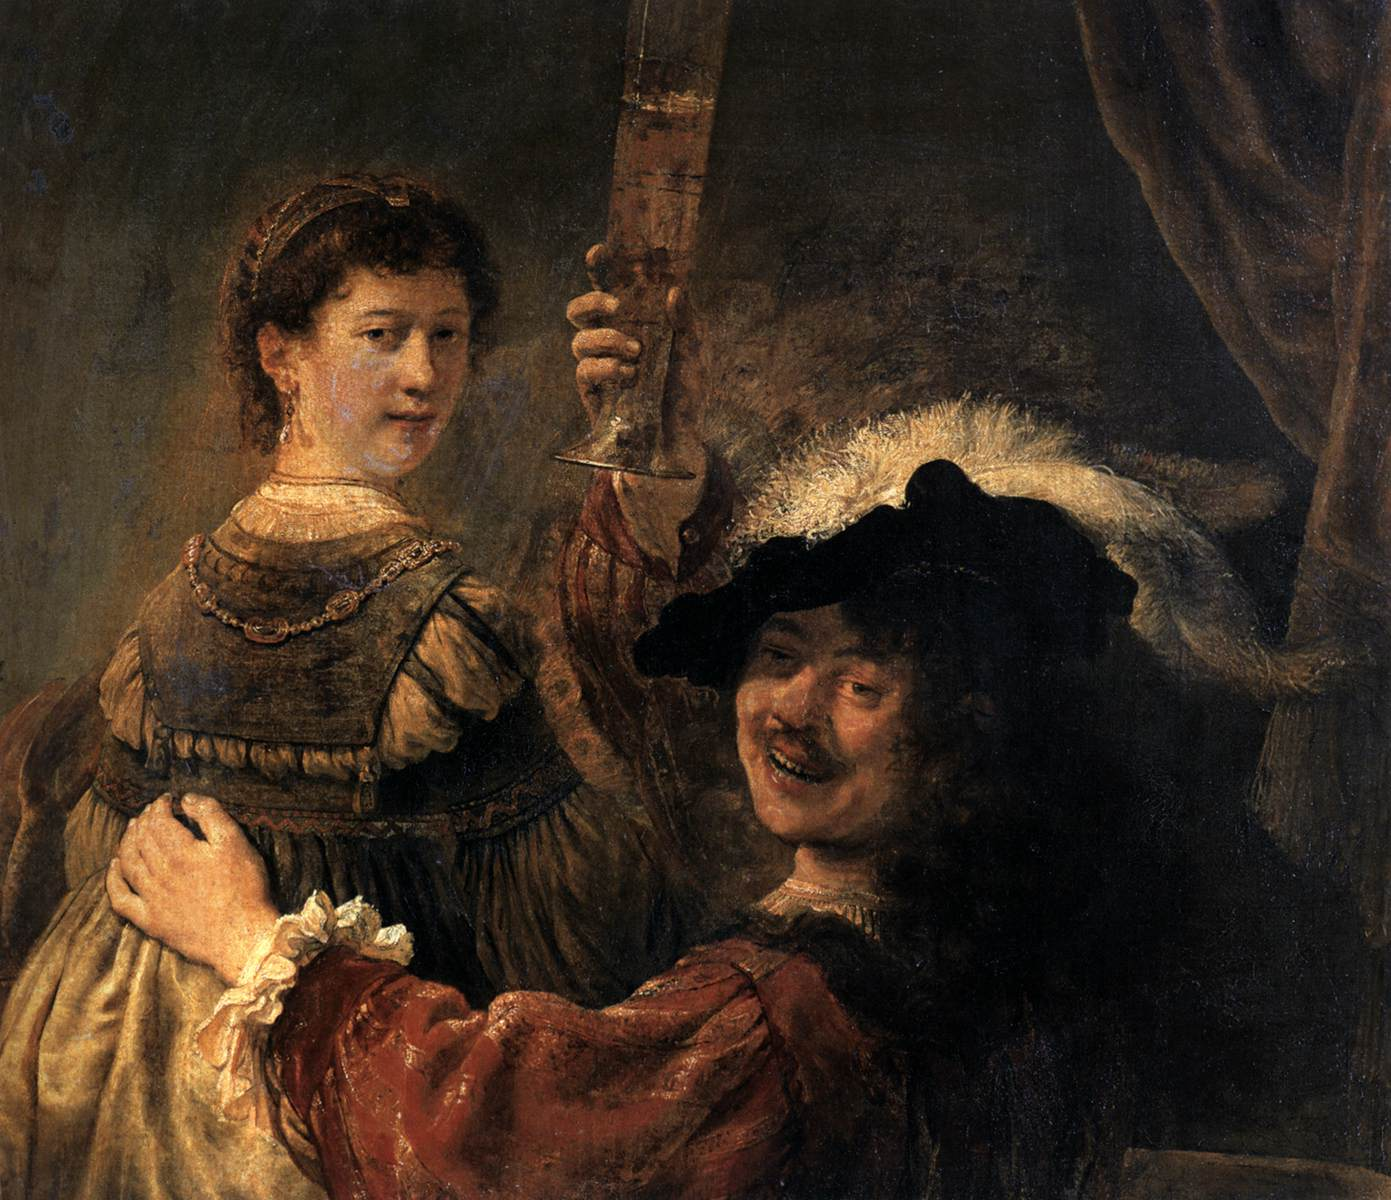
\includegraphics[width=.5in, height=.7in]{pictures/Datasets/art/rembrandt/Gogh283.jpg}
    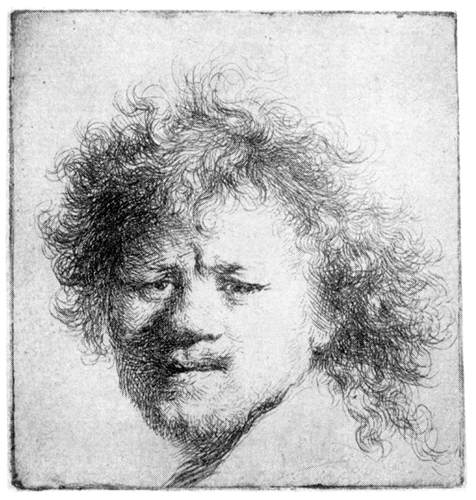
\includegraphics[width=.5in, height=.7in]{pictures/Datasets/art/rembrandt/Gogh303.jpg}
    \includegraphics[width=.5in, height=.7in]{pictures/Datasets/art/rembrandt/Gogh337.jpg}
    \includegraphics[width=.5in, height=.7in]{pictures/Datasets/art/rembrandt/Gogh418.jpg}
    \includegraphics[width=.5in, height=.7in]{pictures/Datasets/art/rembrandt/Gogh73.jpg}
    \includegraphics[width=.5in, height=.7in]{pictures/Datasets/art/rembrandt/Gogh78.jpg}
    \includegraphics[width=.5in, height=.7in]{pictures/Datasets/art/rembrandt/Gogh466.jpg}
    \caption{\textbf{Rembrandt Dataset} Above is a representative sample of Rembrandt van Rijn's work from this study's dataset as chosen by the authors.}
\end{figure}

\begin{figure}[H]
    \centering
    \includegraphics[width=.5in, height=.7in]{pictures/Datasets/art/VanGogh/Gogh0.jpg}
    \includegraphics[width=.5in, height=.7in]{pictures/Datasets/art/VanGogh/Gogh111.jpg}
    \includegraphics[width=.5in, height=.7in]{pictures/Datasets/art/VanGogh/Gogh207.jpg}
    \includegraphics[width=.5in, height=.7in]{pictures/Datasets/art/VanGogh/Gogh236.jpg}
    \includegraphics[width=.5in, height=.7in]{pictures/Datasets/art/VanGogh/Gogh24.jpg}
    \includegraphics[width=.5in, height=.7in]{pictures/Datasets/art/VanGogh/Gogh303.jpg}
    \includegraphics[width=.5in, height=.7in]{pictures/Datasets/art/VanGogh/Gogh35.jpg}
    \includegraphics[width=.5in, height=.7in]{pictures/Datasets/art/VanGogh/Gogh55.jpg}
    \includegraphics[width=.5in, height=.7in]{pictures/Datasets/art/VanGogh/Gogh76.jpg}
    \includegraphics[width=.5in, height=.7in]{pictures/Datasets/art/VanGogh/Gogh91.jpg}
    \includegraphics[width=.5in, height=.7in]{pictures/Datasets/art/VanGogh/Gogh120.jpg}
    \includegraphics[width=.5in, height=.7in]{pictures/Datasets/art/VanGogh/Gogh63.jpg}
    \caption{\textbf{Van Gogh Dataset} Above is a representative sample of Vincent Van Gogh's work from this study's datase tas chosen by the authors.}
\end{figure}

\begin{figure}[H]
    \centering
    \includegraphics[width=3.5in]{pictures/Datasets/art/contStyleCircledCrop.png}
    \includegraphics[width=3.5in]{pictures/Datasets/art/contReference.png}
    \caption{\textbf{Style Expos\'e: Chiaroscuro} InfoGAN captured the artistic style of art labeled as Chiaroscuro - or the contrast of light and shadow to hightlight a subject.  Rembrandt used this technique frequently in his portraits and infoGAN discovered and generated that motif to the viewer.  Under the generated images are sample photos from the Rembrandt dataset that highlights Chiaroscuro.}
\end{figure}

\section{Architecture}

In table 9, we list the dimensions of the input, convolutional, and fully connected layers for $D$, $G$, and $Q$.  The generator accepts the dimensional map $X$ which is a random variable representing the mapping function.  The input then basses through multiple layers that feature ReLU activation functions, and output a 64x64 grayscaled image.  This image is then passed into $D$, which works backwards and outputs the probability scalar.

%Table describing discrim/generator CNNs:
\begin{table}[!h]
\caption{Discriminator and Generator CNNs used across all datasets}
\centering
    \begin{tabular}{ |p{4cm}|p{4cm}|  }
     \hline
     \textbf{Discriminator} $D$ and \textbf{Recognition network} $Q$ & \textbf{Generator} $G$\\
     \hline
     \hline
     Input 64x64 Gray image &Input X dimensional map\\
     \hline
     4 x 4 conv. 64 IRELU. stride 2 \& angled & FC. 1024 RELU. batchnorm \\
     \hline
     4 x 4 conv. 128 IRELU. stride 2. batchnorm& FC. 8 x 8 x 256 RELU. batchnorm \\
     \hline
     4 x 4 conv. 256 IRELU. stride 2. batchnorm& 4 x 4 upconv. 256 RELU. batchnorm \\
     \hline
     4 x 4 conv. 256 IRELU. batchnorm & 4 x 4 upconv. 256 RELU. batchnorm \\
     \hline
     4 x 4 conv. 256 IRELU. batchnorm &4 x 4 upconv. 128 RELU. stride 2. batchnorm \\
     \hline
     FC. 1024 IRELU. batchnorm&4 x 4 upconv. 64 RELU. stride 2. batchnorm \\
     \hline
     FC. output layer&4 x 4 upconv. 1 sigmoid.\\
     \hline
    \end{tabular}
\end{table}


%\vfill

% Can be used to pull up biographies so that the bottom of the last one
% is flush with the other column.
%\enlargethispage{-5in}



\end{document}